\documentclass[a4paper]{scrartcl}
\usepackage[utf8]{inputenc}
\usepackage[english]{babel}
\usepackage{pgfplots}
\usepackage{amsmath, enumerate, amssymb, multirow, fancyhdr, color, graphicx, lastpage, listings, tikz, pdflscape, subfigure, float, polynom, hyperref, tabularx, forloop, geometry, listings, fancybox, tikz, forest, tabstackengine, cancel, bbm}
\input kvmacros
\geometry{a4paper,left=3cm, right=3cm, top=3cm, bottom=3cm}
\pagestyle {fancy}


\begin{document}


We assume $\sigma$ is the weight matrix of a weighted undirected graph, so $\sigma_{ij} = \sigma_{ji}$ and $\sigma_{ij} = 1$ if there is an edge between $i$ to $j$ and $\sigma_{ij} = 0$ if there is no edge between $i$ and $j$.
For simplicity we assume that nodes are not self connected, that is $\sigma_{ii} = 0$.

\section*{(a)}

{
\color{green}
TODO: Note the $\leq$ instead of the $=$ in the following. This propagates through all formulas below!
}

For $M$ to be a matching, it needs to hold by definition, that $$\forall i:  \sum_j \sigma_{ij} \leq 1$$ 
This is equivalent to saying $$ \prod_i \mathbbm{1}_{\left[\sum_j \sigma_{ij} \leq 1\right]} = 1 $$
where $\mathbbm{1}$ is the indicator function.

So we find the probability distribution

\begin{align}
    P(M) = \frac{1}{Z}\prod_i \mathbbm{1}_{\left[\sum_j \sigma_{ij} \leq 1\right]}
\end{align}

Where $Z$ is the normalization wich is the count of all matchings 
\begin{align}
    Z = \sum_{M \in \mathcal{G}} \mathbbm{1}_{\left[ \prod_i \mathbbm{1}_{\left[\sum_j \sigma_{ij} \leq 1\right]} = 1 \right]} 
\end{align}
Here $\mathcal{G}$ is the set of all subsets of the graph.

\section*{(b)}

The size of a matching $\lvert M \rvert$ is the count of its edges. With the adjecency matrix $\sigma$ that is the sum of all its elements divided by two: $$ \lvert M \rvert = \frac{\sum_{i} \sum_{j} \sigma_{ij}}{2}$$

We simply introduce the size of a matching $\lvert M \rvert$ as a scaling factor in the probability distribution, to give larger weight to larger matchings:

\begin{align}
    P(M) = \frac{1}{Z} \lvert M \rvert \prod_i \mathbbm{1}_{\left[\sum_j \sigma_{ij} \leq 1\right]}
\end{align}

which has new normalization factor

\begin{align}
    Z = \sum_{M \in \mathcal{G}} \lvert M \rvert \cdot \mathbbm{1}_{\left[ \prod_i \mathbbm{1}_{\left[\sum_j \sigma_{ij} \leq 1\right]} = 1 \right]} 
\end{align}



% We have the size $S = M=\sum_{ij} \sigma^{ij}$ and the normalized version $S^*=\frac{M}{\lvert E \rvert}$.

{\color{red}
TODO I feel like there would be a way to integrate the scalar $\lvert M \rvert$ into the factor (in the product) but i can't find it. (Nevermind i don't think so anymore, with clarification 2 we don't need it anyways)
}

\section*{(c)}

The Graph is given as:

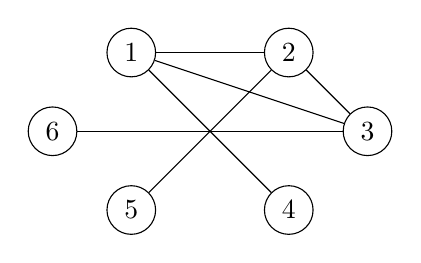
\begin{tikzpicture}
    [scale=1,auto=left,every node/.style={circle,draw}]
    \node (n1) at (1,3) {1};
    \node (n2) at (3,3)  {2};
    \node (n3) at (4,2)  {3};
    \node (n4) at (3,1) {4};
    \node (n5) at (1,1)  {5};
    \node (n6) at (0,2)  {6};
  
    \foreach \from/\to in {n1/n2,n1/n3,n2/n3,n1/n4,n2/n5,n3/n6}
      \draw (\from) -- (\to);
  
\end{tikzpicture}

An ordered drawing of this graph is:


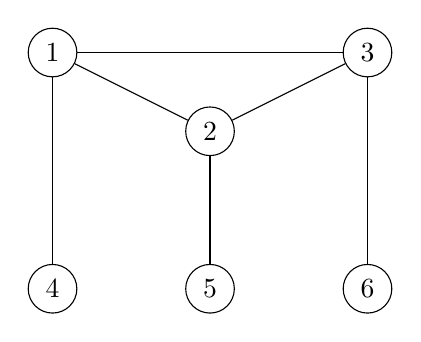
\begin{tikzpicture}
    [scale=1,auto=left,every node/.style={circle,draw}]
    \node (n1) at (1,4) {1};
    \node (n2) at (3,3)  {2};
    \node (n3) at (5,4)  {3};
    \node (n4) at (1,1) {4};
    \node (n5) at (3,1)  {5};
    \node (n6) at (5,1)  {6};
  
    \foreach \from/\to in {n1/n2,n1/n3,n2/n3,n1/n4,n2/n5,n3/n6}
      \draw (\from) -- (\to);
  
\end{tikzpicture}
  





In general the probability distribution found above is given as
\begin{align}
    P(M) = \frac{1}{Z}\prod_i \mathbbm{1}_{\left[\sum_j \sigma_{ij} \leq 1\right]}
\end{align}
Which we can write as 
\begin{align}
    P(M) = \frac{1}{Z} \prod_i \psi_i(\partial M)
\end{align}
with factors
\begin{align}
    \psi_i(\partial M) = \mathbbm{1}_{\left[ \sum_j \sigma_{ij} \leq 1 \right]}
\end{align}

By $\partial M$ we denote, that each factor $\psi_i$ is only connected to all nodes $\sigma_{ij}$ for which there is a connection from $i$ to $j$, so for all nodes for which $\sigma_{ij} = 1$ in the initial graph $G$.


In general to draw a factor graph we would start with a graph with all $\sigma_{ij}$ connected to all factors $\psi_i$. Then we can omit all $\sigma_{ij}$ where $\sigma_{ij} = 0$ in the initial graph $G$. Furthermore we can omit all connections from factors $\psi_i$ to $\sigma_{ij}$ if $i$ and $j$ are not connected. 

For the graph given here this yields the factor graph:

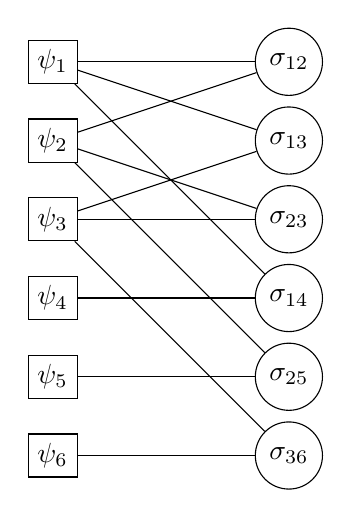
\begin{tikzpicture}
    [scale=1,auto=left,every node/.style={circle,draw}]
    \node (s12) at (4,6) {$\sigma_{12}$};
    \node (s13) at (4,5) {$\sigma_{13}$};
    \node (s23) at (4,4) {$\sigma_{23}$};
    \node (s14) at (4,3) {$\sigma_{14}$};
    \node (s25) at (4,2) {$\sigma_{25}$};
    \node (s36) at (4,1) {$\sigma_{36}$};
  
    \node[rectangle] (f1) at (1,6) {$\psi_{1}$};
    \node[rectangle] (f2) at (1,5) {$\psi_{2}$};
    \node[rectangle] (f3) at (1,4) {$\psi_{3}$};
    \node[rectangle] (f4) at (1,3) {$\psi_{4}$};
    \node[rectangle] (f5) at (1,2) {$\psi_{5}$};
    \node[rectangle] (f6) at (1,1) {$\psi_{6}$};
  


    \foreach \from/\to in {f1/s12,f1/s13,f1/s14,f2/s12,f2/s23,f2/s25,f3/s13,f3/s23,f3/s36,f4/s14,f5/s25,f6/s36}
      \draw (\from) -- (\to);
  
\end{tikzpicture}



{\color{red}
TODO Is this also so simple for the probability distribution scaled by matching size $\lvert M \rvert$? (Nevermind, is saw Clarification 2)
}











\section*{(d)}

The general definitions are given as:
\begin{align}
    \nu_{i \rightarrow a}^{(t + 1)}(x_i) &\cong \prod_{b \in \partial i \backslash a} \hat{\nu}_{b \rightarrow i}^{(t)}(x_i) \\
    \hat{\nu}_{a \rightarrow i}^{(t)}(x_i) &\cong \sum_{\textbf{x}_{\partial a} \backslash i} \psi_a (\textbf{x}_{\partial a}) \prod_{j \in \partial a \backslash i} \nu_{j \rightarrow a}^{(t)}(x_j) \\
    P(x_i) &= \nu_i^{(t)}(x_i) \cong \prod_{a \in \partial i} \hat{\nu}_{a \rightarrow i}^{(t-1)}(x_i)
\end{align}


In our case we have messages from variable to factor:
\begin{align}
    \nu_{\sigma_{ij}}^{(ij) \rightarrow i} \cong \prod_{b \in \partial (ij) \backslash i} \hat{\nu}_{\sigma_{ij}}^{b \rightarrow (ij)}
\end{align}
and factor to variable:
\begin{align}
    \hat{\nu}_{\sigma_{ij}}^{i \rightarrow (ij)} \cong \sum_{\boldsymbol{\sigma}_{\partial i} \backslash (ij)} 
    \psi_i(\boldsymbol{\sigma}_{\partial i}) \prod_{(ik) \in \partial i \backslash (ij)} \nu_{\sigma_{ik}}^{(ik) \rightarrow i}
\end{align}

For our problem this leads to messages from factor to variable:
\begin{align}
    \hat{\nu}_{\sigma_{ij}}^{i \rightarrow (ij)} &\cong \sum_{\sigma_{\partial i} \backslash (ij)} \mathbbm{1}_{\left[\sum_l \sigma_{il} \leq 1 \right]} \prod_{(ik) \in \partial i \backslash (ij)} \nu_{\sigma_{ik}}^{(ik) \rightarrow i}\\
\end{align}

This means the marginal is:
\begin{align}
    P(\sigma_{ij}) &\cong \prod_{b \in \partial (ij)} \hat{\nu}_{\sigma_{ij}}^{b \rightarrow (ij)} \\
    &= \hat{\nu}_{\sigma_{ij}}^{i \rightarrow (ij)} \cdot \hat{\nu}_{\sigma_{ij}}^{j \rightarrow (ij)}
\end{align}



{
\color{green}
TODO: I don't know if we have to write something for the second hint, but this would be the following?
}

In the following we find some derivations for the adjecent edges if $\sigma_{ij} = 1$ and $\sigma_{ij} = 0$:

For $\sigma_{ij} = 1$ this leads to 
\begin{align}
    P(\sigma_{ij} = 1) &\cong \hat{\nu}_{\sigma_{ij}}^{i \rightarrow (ij)} \cdot \hat{\nu}_{\sigma_{ij}}^{j \rightarrow (ij)} \\
    &= \left[ \sum_{\sigma_{\partial i} \backslash (ij)} \mathbbm{1}_{\left[\sum_l \sigma_{il} \leq 1 \right]} \prod_{(ik) \in \partial i \backslash (ij)} \nu_{\sigma_{ik}}^{(ik) \rightarrow i} \right]
     \cdot \left[ \sum_{\sigma_{\partial j} \backslash (ij)} \mathbbm{1}_{\left[\sum_l \sigma_{jl} \leq 1 \right]} \prod_{(jk) \in \partial j \backslash (ij)} \nu_{\sigma_{jk}}^{(jk) \rightarrow j} \right]
\end{align}
Which can only be $\geq 0$ if 
\begin{align}
    \sum_{\sigma_{\partial i} \backslash (ij)} \mathbbm{1}_{\left[\sum_l \sigma_{il} \leq 1 \right]} &= 1 \\
    \sum_{\sigma_{\partial i} \backslash (ij)} \mathbbm{1}_{\left[\sum_{l \backslash (l = j)} \sigma_{il} + 1 \leq 1 \right]} &= 1 \\
\end{align}
and 
\begin{align}
    \sum_{\sigma_{\partial j} \backslash (ij)} \mathbbm{1}_{\left[\sum_l \sigma_{jl} \leq 1 \right]} &= 1 \\
    \sum_{\sigma_{\partial j} \backslash (ij)} \mathbbm{1}_{\left[\sum_{l \backslash (l = i)} \sigma_{jl} + 1 \leq 1 \right]} &= 1
\end{align}

This is saying that all edges adjecent to $i$ and $j$ except edge $(ij)$ have to be zero, meaning non existant. 


For $\sigma_{ij} = 0$ we find with similar reasoning:

\begin{align}
    P(\sigma_{ij} = 0) &\cong \hat{\nu}_{\sigma_{ij}}^{i \rightarrow (ij)} \cdot \hat{\nu}_{\sigma_{ij}}^{j \rightarrow (ij)} \\
    &= \left[ \sum_{\sigma_{\partial i} \backslash (ij)} \mathbbm{1}_{\left[\sum_l \sigma_{il} \leq 1 \right]} \prod_{(ik) \in \partial i \backslash (ij)} \nu_{\sigma_{ik}}^{(ik) \rightarrow i} \right]
     \cdot \left[ \sum_{\sigma_{\partial j} \backslash (ij)} \mathbbm{1}_{\left[\sum_l \sigma_{jl} \leq 1 \right]} \prod_{(jk) \in \partial j \backslash (ij)} \nu_{\sigma_{jk}}^{(jk) \rightarrow j} \right]
\end{align}
Which can only be $\geq 0$ if 
\begin{align}
    \sum_{\sigma_{\partial i} \backslash (ij)} \mathbbm{1}_{\left[\sum_l \sigma_{il} \leq 1 \right]} &= 1 \\
    \sum_{\sigma_{\partial i} \backslash (ij)} \mathbbm{1}_{\left[\sum_{l \backslash (l = j)} \sigma_{il} + 0 \leq 1 \right]} &= 1 \\
\end{align}
and 
\begin{align}
    \sum_{\sigma_{\partial j} \backslash (ij)} \mathbbm{1}_{\left[\sum_l \sigma_{jl} \leq 1 \right]} &= 1 \\
    \sum_{\sigma_{\partial j} \backslash (ij)} \mathbbm{1}_{\left[\sum_{l \backslash (l = i)} \sigma_{jl} + 0 \leq 1 \right]} &= 1
\end{align}

Which is saying that any one, but no more than one of the edges adjecent to $i$ except $(ij)$ may be 1 and that any one, but no more than one of the edges adjecent to $j$ except $(ij)$ may be 1. 
If we use $c_i$ and $c_j$ as the count of edges adjecent to $i$ and $j$ except for edge $(ij)$ respectively, we can say that this allows $c_i+1$ configurations for the edges adjecent to $i$ and $c_j + 1$ configurations for the edges adjecent to $j$ (Any one may be 1 or all are 0).

These derivations are intuitively consistent with the definitions of the matching.





{
\color{green}
TODO i don't quite get the following, from the reasoning it makes sense but i don't see how it follows from the formulas


For $\sigma_{ij}=1$, this leads to:
\begin{align}
    P(\sigma_{ij}=1) =  \prod_{\sigma_{ik} \in \partial a \backslash i} v_{\sigma_{ik} \rightarrow i}(0)
\end{align}
wich intuitively makes sense, since all the others have to be 0 in order for $\sigma_{ij}$ to be 1.\\
For $\sigma_{ij}=0$, this leads to:
\begin{align}
    P(\sigma_{ij}=1) = \sum_{\sigma_{ik} \in \partial i \backslash \sigma_{ij}} (\mathbbm{1}^{(\sum_{l \backslash i} \sigma_{il} = 1)} \prod_{\sigma_{ik} \in \partial a \backslash i} v_{\sigma_{ik} \rightarrow i}(\sigma_{ik}))\\
\end{align}
here the main difference is that the factor $\Psi_{i}$ doesn't sum over $\sigma_{ij}$ anymore, since it is set to 0.
}





{
\color{red}
We have the messages from variable to factor:
\begin{align}
    \hat{v}_{i \rightarrow \alpha}(x_i) = \prod_{\beta \in \partial \alpha \backslash i} \hat{v}_{b \rightarrow i}(x_i)
\end{align}
and factor to variable:
\begin{align}
    \hat{v}_{\alpha \rightarrow i}(x_i) = \sum_{x \in \partial \alpha \backslash i} (\Psi_a(X_{\partial a}) \prod_{j \in \partial a \backslash i} v_{j \rightarrow a}(x_j))
\end{align}

The general BP marginal is:
\begin{align}
    P(x_i) = v_i(x_i) = \prod_{a \in \partial i} \hat{v}_{\alpha \rightarrow i}(x_i)
\end{align}

For our problem, this leads to to message from factor to variable:
\begin{align}
    \hat{v}_{i \rightarrow \sigma_{ij}}(\sigma_{ij}) &= \sum_{\sigma_{ik} \in \partial i \backslash \sigma{ij}} (\mathbbm{1}^{(\sum_l \sigma^{il} = 1)} \prod_{\sigma_{ik} \in \partial a \backslash i} v_{\sigma_{ik} \rightarrow i}(\sigma_{ik}))\\
\end{align}

This means the marginal is:
\begin{align}
    P(\sigma_{ij}) = \hat{v}_{i \rightarrow \sigma_{ij}}(\sigma_{ij}) \cdot \hat{v}_{j \rightarrow \sigma_{ij}}(\sigma_{ij})
\end{align}
For $\sigma_{ij}=1$, this leads to:
\begin{align}
    P(\sigma_{ij}=1) =  \prod_{\sigma_{ik} \in \partial a \backslash i} v_{\sigma_{ik} \rightarrow i}(0)
\end{align}
wich intuitively makes sense, since all the others have to be 0 in order for $\sigma_{ij}$ to be 1.\\
For $\sigma_{ij}=0$, this leads to:
\begin{align}
    P(\sigma_{ij}=1) = \sum_{\sigma_{ik} \in \partial i \backslash \sigma_{ij}} (\mathbbm{1}^{(\sum_{l \backslash i} \sigma_{il} = 1)} \prod_{\sigma_{ik} \in \partial a \backslash i} v_{\sigma_{ik} \rightarrow i}(\sigma_{ik}))\\
\end{align}
here the main difference is that the factor $\Psi_{i}$ doesn't sum over $\sigma_{ij}$ anymore, since it is set to 0.


}






\section*{(d)}
{
\color{green}
TODO: To get the full marginal we would need to do the full message passing. For the equations the following suffices:

}

For one point marginal, see (c):
\begin{align}
    P(\sigma_{ij}) &\cong \hat{\nu}_{\sigma_{ij}}^{i \rightarrow (ij)} \cdot \hat{\nu}_{\sigma_{ij}}^{j \rightarrow (ij)}
\end{align}


For two point marginal, we have:
\begin{align}
    P(\sigma_{ij}, \sigma_{kl}) = P(\sigma_{kl} \vert \sigma_{ij}) P(\sigma_{ij})
\end{align}

In addition to the one point marginal we need to  find $P(\sigma_{kl} \vert \sigma_{ij})$ which is defined by:
\begin{align}
    P(\sigma_{kl} \vert \sigma_{ij} = x) &\cong \prod_{a} \psi_a(\boldsymbol{\sigma}_{\partial a}) \mathbbm{1}_{\left[ \sigma_{ij} = x \right]} \\
    &= \prod_{a} \mathbbm{1}_{\left[ \sum_{l} \sigma_{al} \leq 1 \right]} \mathbbm{1}_{\left[ \sigma_{ij} = x \right]}
\end{align}

This is, we add to the original factor graph a node of degree 1 connected to the variable node $\sigma_{ij}$ which fixes $\sigma_{ij} = x$ and run BP on this modified factor graph.




\end{document}

